\documentclass[12pt]{article}

\usepackage[T1]{fontenc}
\usepackage[utf8]{inputenc}
\usepackage{lmodern}
\usepackage[margin=2.3cm]{geometry}
\usepackage{amsmath,amssymb}
\usepackage{booktabs,tabularx,longtable}
\usepackage{array}
\usepackage[dvipsnames]{xcolor}
\usepackage{tikz}
\usetikzlibrary{arrows.meta,positioning,calc,shapes.geometric,fit}
\usepackage{algorithm}
\usepackage[noend]{algpseudocode}
\usepackage[most]{tcolorbox}
\usepackage{enumitem}
\usepackage{microtype}
\usepackage{float}
\usepackage{hyperref}
\hypersetup{colorlinks=true,linkcolor=NavyBlue,urlcolor=NavyBlue,citecolor=NavyBlue}

% ------------------------------------------------------------------ styling
\definecolor{galaxyc}{RGB}{40,90,170}
\definecolor{sunc}{RGB}{200,110,0}
\definecolor{corec}{RGB}{30,130,70}

\newcommand{\GALAXY}{\textcolor{galaxyc}{\textbf{\textsf{GALAXY}}}}
\newcommand{\SUN}{\textcolor{sunc}{\textbf{\textsf{SUN}}}}
\newcommand{\SINGLE}{\textbf{\textsf{SINGLE}}}
\newcommand{\TWO}{\textbf{\textsf{TWO}}}
\newcommand{\opt}[1]{\texttt{-{}-#1}}
\newcommand{\vect}[1]{\mathbf{#1}}
\newcommand{\gperp}{g_{\perp}}

\newtcolorbox{galaxybox}[1][]{enhanced,breakable,colback=galaxyc!6,colframe=galaxyc,
  fonttitle=\bfseries\sffamily,title={GALAXY mode#1},left=4pt,right=4pt,top=3pt,bottom=3pt}
\newtcolorbox{sunbox}[1][]{enhanced,breakable,colback=sunc!7,colframe=sunc,
  fonttitle=\bfseries\sffamily,title={SUN mode#1},left=4pt,right=4pt,top=3pt,bottom=3pt}
\newtcolorbox{corebox}[1][]{enhanced,breakable,colback=corec!6,colframe=corec,
  fonttitle=\bfseries\sffamily,title={#1},left=4pt,right=4pt,top=3pt,bottom=3pt}

\algrenewcommand\algorithmicrequire{\textbf{Input:}}
\algrenewcommand\algorithmicensure{\textbf{Output:}}
\algnewcommand{\IfSun}[1]{\State \textcolor{sunc}{\textsf{[SUN]}}~#1}
\algnewcommand{\IfGal}[1]{\State \textcolor{galaxyc}{\textsf{[GALAXY]}}~#1}
\algblockdefx[ParFor]{ParFor}{EndParFor}[1]{\textbf{parallel for} #1 \textbf{do}}{}
\algnewcommand\LComment[1]{\State \(\triangleright\) \textit{#1}}

\setlist{itemsep=2pt,topsep=4pt}
\setlength{\parskip}{3pt}

\title{\textbf{Dark matter from self-interacting gravitational field lines}\\[4pt]}
\author{}
\date{}

\begin{document}
\maketitle

\begin{abstract}
This document describes a C++/OpenGL program that simulates gravitational \emph{field lines}, which are themselves sources of gravity. 
The lines are deposited onto a 3D grid as a mass density, the Poisson equation
is solved for the potential, and the resulting gravitational acceleration
bends the same lines in the next step. The field therefore acts back on the
lines that produce it: gravity is \emph{self-interacting}. The program offers
four modes. This document concentrates on the self-interaction loop and on
the two modes that differ most, \GALAXY\ (many emitters, normalized bending, flat rotation curves) and \SUN\ (one body at physical scale, interior chords, physical bending, mass measurement, Keplerian falloff). 
All procedures are given as algorithms rather than source code.
\end{abstract}

%\setcounter{tocdepth}{1}
%\tableofcontents

% ==================================================================
\section{Overview}
% ==================================================================

The program (\url{https://github.com/sjhalayka/dark_matter}) 
simulates many different scenes. is a single translation unit of 
about 2100 lines. It splits into five functional layers:

\begin{enumerate}
  \item \textbf{Geometry and encoding.} A small vector type, a 16-byte packed
        node (position plus an octahedrally encoded direction) and a
        counter-based hashing random number generator.
  \item \textbf{The simulation class \texttt{Sim}.} It holds the emitters, the
        field-line store, the density/potential/acceleration grids and the
        step loop. This is where self-interacting gravity happens.
  \item \textbf{The grid solver.} It applies a Dirichlet monopole boundary, runs
        red--black successive over-relaxation (SOR) for $\nabla^2\phi = 4\pi\rho$
        and takes a central-difference gradient. There is a multithreaded CPU
        version and an OpenGL~4.3 compute-shader version.
  \item \textbf{Diagnostics.} Rotation curves (all modes) and, in \SUN\ mode only,
        a mass measurement from chord statistics, light deflection, Shapiro delay
        and Gauss's law.
  \item \textbf{Visualization.} Line clouds, highlighted lines, a ray-marched
        density volume, exterior field streamlines (\SUN), PNG screenshots and
        an interactive camera.
\end{enumerate}

Two threads run concurrently. The \emph{simulation thread} calls
\texttt{Sim::step()} repeatedly and serves diagnostic requests between steps.
The \emph{GL thread} owns the OpenGL context: it renders, and on request it
runs the GPU Poisson solve for the simulation thread (Section~\ref{sec:gpu}).

\subsection{The central idea: lines that gravitate}

In the conventional picture a mass produces a field, and field lines are only
a way of drawing that field. Here the relation is reversed. Each emitter owns
$n$ field lines (default $n=10^4$), and the \emph{length of line per unit
volume} is the mass density. A straight radial line contributes density
$\propto 1/r^2$, so a field-line cloud is a gravitating halo. Its own field
bends the lines. The bent lines then deposit a different density, which gives
a different field, and so on. The program iterates this loop until it reaches a
quasi-steady state, or for as long as the user lets it run.

The emitter radius is linked to $n$ by a holographic counting rule: one field
line per $4\ln 2$ Planck areas of horizon,
\begin{equation}
  n = \frac{4\pi R^2}{4\ln 2}
  \quad\Longrightarrow\quad
  R = \sqrt{\frac{n\ln 2}{\pi}}
  \label{eq:radius}
\end{equation}
in Planck lengths. 
$n$ is also known as binary entropy. 
For $n = 10^4$ this gives $R\approx 46.97$. In \SINGLE, \TWO\ and
(nominally) \GALAXY\ mode the length unit is the Planck length, and $R$ is the
Schwarzschild radius of the $n$ lines. In \SUN\ mode the same relation is used,
but each simulated line stands for many real lines and lengths are rescaled
(Section~\ref{sec:sun}).
% ==================================================================
\section{Data structures}
% ==================================================================

\subsection{Packed nodes}

A field line is a chain of nodes. Each node stores its position and the unit
direction of the segment \emph{that ends at it}. Positions are three 32-bit
floats. The direction uses \emph{octahedral encoding}, compressed to two signed
16-bit integers, so a node takes exactly 16 bytes.

\begin{algorithm}[htbp]
\caption{Octahedral direction encoding (\texttt{packNode} / \texttt{unpackNode})}
\begin{algorithmic}[1]
\Function{Pack}{$\vect p, \vect v$}
  \State $s \gets |v_x|+|v_y|+|v_z|$; \quad $(x,y)\gets(v_x/s,\, v_y/s)$
     \Comment{project onto the octahedron $|x|+|y|+|z|=1$}
  \If{$v_z<0$} \Comment{fold the lower hemisphere outward}
     \State $(x,y)\gets\big((1-|y|)\,\mathrm{sgn}(x),\ (1-|x|)\,\mathrm{sgn}(y)\big)$
  \EndIf
  \State \Return $(\vect p,\ \mathrm{round}(32767\,\mathrm{clamp}(x)),\ \mathrm{round}(32767\,\mathrm{clamp}(y)))$
\EndFunction
\Function{Unpack}{$\vect p, o_0, o_1$}
  \State $x\gets o_0/32767$, $y\gets o_1/32767$, $z\gets 1-|x|-|y|$, $t\gets\max(-z,0)$
  \State $x \gets x - t\,\mathrm{sgn}(x)$; \quad $y\gets y - t\,\mathrm{sgn}(y)$
  \State \Return $(\vect p,\ \mathrm{normalize}(x,y,z))$
\EndFunction
\end{algorithmic}
\end{algorithm}

The angular resolution is about $3\times10^{-5}$\,rad, which is far finer than
the per-step bending angles in all modes except \SUN.

\subsection{Line-major node store}

All lines of all emitters are stored one after another in a byte stream. Each
line is written as a 32-bit node count followed by that many packed nodes. The
order is fixed: line id $= e\cdot n + i$ for emitter $e$ and line $i$. Every step
reads the store from the previous step and writes a new one (double buffering).
If the estimated steady-state size
\[
  B \approx N_\text{lines}\cdot\frac{2H_\text{max}}{\ell}\cdot 16 + 4N_\text{lines}\ \text{bytes}
\]
exceeds the RAM budget (\opt{ram}, default 24\,GB), the two buffers become two
swap files on disk. Otherwise they are two in-memory byte vectors. Here $\ell$ is
the segment length and $H_\text{max}$ is the largest box half-size.

\subsection{Grids}

The simulation box $[-H_x,H_x]\times[-H_y,H_y]\times[-H_z,H_z]$ is divided into
$N_x\times N_y\times N_z$ cells. With \opt{grid} given as a single value the cells are
cubic, and the longest axis gets that many cells (default 250). Five
float grids are kept: $\rho$, $\phi$, $g_x$, $g_y$, $g_z$. In addition, each
thread has a private density grid so that deposition needs no atomics. All are
indexed $i + N_x j + N_xN_y k$.

\subsection{Deterministic randomness}

The program has no random state. Every random quantity is a hash of an identifier
through SplitMix64, so a line's starting point and direction can be
recomputed from its id at any time. This is how a line is rebuilt from its
origin every step without storing the origin. Uniform points on the unit
sphere come from $(u,v)\mapsto(\sqrt{1-z^2}\cos 2\pi v,\ \sqrt{1-z^2}\sin 2\pi v,\ z)$
with $z = 2u-1$.

% ==================================================================
\section{The self-interaction loop}
\label{sec:loop}
% ==================================================================

This section is the core of the program. One call to \texttt{Sim::step()}
advances every line by one segment and recomputes the gravitational field
from all lines together. Figure~\ref{fig:cycle} shows the cycle.

\begin{figure}[htb]
\centering
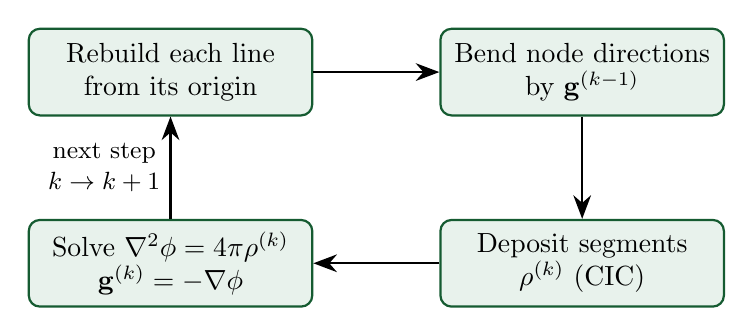
\begin{tikzpicture}[
  box/.style={draw,rounded corners,align=center,minimum width=3.6cm,minimum height=1.1cm,fill=#1!10,draw=#1!70!black,thick},
  box/.default=corec,
  arr/.style={-{Stealth[length=3mm]},thick}]
\node[box] (rebuild) {Rebuild each line\\from its origin};
\node[box,right=1.6cm of rebuild] (kick) {Bend node directions\\by $\vect g^{(k-1)}$};
\node[box,below=1.3cm of kick] (dep) {Deposit segments\\$\rho^{(k)}$ (CIC)};
\node[box,below=1.3cm of rebuild] (pois) {Solve $\nabla^2\phi=4\pi\rho^{(k)}$\\$\vect g^{(k)}=-\nabla\phi$};
\draw[arr] (rebuild) -- (kick);
\draw[arr] (kick) -- (dep);
\draw[arr] (dep) -- (pois);
\draw[arr] (pois) -- node[left,align=center,font=\small]{next step\\$k\to k+1$} (rebuild);
\node[font=\small,align=center,text width=4cm] at ($(rebuild)!0.5!(dep)$) {};
\end{tikzpicture}
\caption{One step of the self-interacting field-line simulation. The field
used to bend the lines in step $k$ comes from the lines of step $k-1$, which is an
explicit (lagged) coupling.}
\label{fig:cycle}
\end{figure}

\subsection{Line growth by ``aging''}

A line is not integrated from start to end in one go. It grows by one node per step:
\begin{itemize}
  \item The new node~0 is always the emitter-surface start point
        $\vect p_0$, with the start direction $\vect d_0$ recomputed from the hash.
  \item Old node $j$ becomes new node $j+1$. Only its \emph{direction} is reused
        (after bending). Its position is recomputed as
        $\vect p_{j+1} = \vect p_j + \ell\,\vect v_j$.
\end{itemize}
The chain is therefore always connected and anchored to the emitter. A change in
direction at an inner node moves every node outside it. After $k$ steps a line
has at most $k+1$ nodes. It stops growing when its next node would leave the
box, enter the body surface (\SUN), or enter another emitter (with
\opt{end-at-emitters}). The deposited density approaches its steady-state
form as the lines fill the box, which takes about $H/\ell$ steps.

\begin{figure}[htb]
\centering
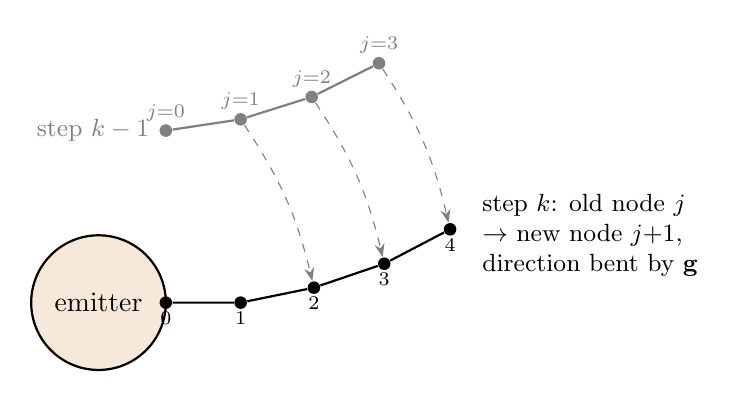
\begin{tikzpicture}[scale=0.95,
  nd/.style={circle,fill=#1,inner sep=1.6pt}, nd/.default=black]
\draw[thick,fill=sunc!15] (0,0) circle (0.9);
\node at (0,0) {emitter};
% old line
\foreach \i/\x/\y in {0/0.9/0,1/1.9/0.15,2/2.85/0.45,3/3.75/0.9}
  \node[nd=gray] (o\i) at (\x,\y+2.3) {};
\draw[gray,thick] (o0)--(o1)--(o2)--(o3);
\node[gray,left] at (o0.west) {\small step $k-1$};
\foreach \i in {0,...,3} \node[gray,above,font=\scriptsize] at (o\i) {$j{=}\i$};
% new line
\foreach \i/\x/\y in {0/0.9/0,1/1.9/0,2/2.88/0.2,3/3.82/0.52,4/4.7/0.98}
  \node[nd] (n\i) at (\x,\y) {};
\draw[thick] (n0)--(n1)--(n2)--(n3)--(n4);
\foreach \i in {0,...,4} \node[below,font=\scriptsize] at (n\i) {\i};
\node[right,align=left,font=\small] at (5,0.9) {step $k$: old node $j$\\$\to$ new node $j{+}1$,\\direction bent by $\vect g$};
\draw[-{Stealth},dashed,gray] (o1) to[bend left=10] (n2);
\draw[-{Stealth},dashed,gray] (o2) to[bend left=10] (n3);
\draw[-{Stealth},dashed,gray] (o3) to[bend left=10] (n4);
\end{tikzpicture}
\caption{Aging of a line. Node~0 is pinned to the emitter. Each old direction is
reused one place further out, and positions are re-chained from the origin.}
\end{figure}

\subsection{The step algorithm}

\begin{algorithm}[htbp]
\caption{\textsc{Step} --- one iteration of self-interacting gravity}
\label{alg:step}
\begin{algorithmic}[1]
\Require node store $S^{(k-1)}$, field $\vect g^{(k-1)}$, $g_\text{ref}=\max|\vect g^{(k-1)}|$
\Ensure node store $S^{(k)}$, density $\rho^{(k)}$, field $\vect g^{(k)}$
\State zero every per-thread density grid $\rho_t$
\State open input stream $S^{(k-1)}$ (absent at $k=0$) and output stream $S^{(k)}$
\If{physical bending (\SUN\ without \opt{strength})}
   \State $\kappa \gets 2\,G_\text{eff}\,\ell$ \Comment{turn $=2G\gperp\,\ell$ per step}
\Else
   \State $\kappa \gets s/g_\text{ref}$ \Comment{$s=$ \opt{strength}: max turn per step in rad}
\EndIf
\For{each batch of up to \texttt{chunk} ($2^{22}$) lines, in id order}
   \State read the node counts and nodes of the batch from $S^{(k-1)}$
   \ParFor{each line id in the batch, on thread $t$}
      \State \Call{ProcessLine}{id, old nodes, $\kappa$, $\rho_t$} \Comment{Alg.~\ref{alg:line}}
   \EndParFor
   \State append every thread's output to $S^{(k)}$ in thread order (keeps id order)
\EndFor
\State close streams; swap buffers or swap files
\State $\rho \gets \sum_t \rho_t$; \quad $M \gets c_\text{vol}\sum\rho$
\If{mode $\neq$ \SUN} $M\gets M/2$ \Comment{boundary carries half the mass}
\EndIf
\State \Call{SolveField}{$\rho, M$} \Comment{Alg.~\ref{alg:poisson}, CPU or GPU}
\IfSun{trace exterior streamlines for display (Alg.~\ref{alg:stream})}
\State publish display buffers under the display mutex
\end{algorithmic}
\end{algorithm}

Algorithm~\ref{alg:step} gives one complete step. Each thread processes a contiguous block of line ids and appends to its own
output buffer. Writing the buffers in thread order therefore keeps the line-major
order the next step expects. The batch size limits memory use when the
store is on disk.

\subsection{Processing one line}

\begin{algorithm}[htbp]
\caption{\textsc{ProcessLine} --- bend, re-chain, deposit and terminate one line}
\label{alg:line}
\begin{algorithmic}[1]
\Require line id, old nodes $(\vect q_j,\vect v_j)_{j<m}$, bending factor $\kappa$, thread grid $\rho_t$
\State $e\gets\lfloor \text{id}/n\rfloor$; \quad $(\vect p,\vect d_0)\gets$\Call{LineStart}{$e$, id mod $n$} \Comment{Alg.~\ref{alg:start}}
\State emit node $(\vect p,\vect d_0)$; \quad $\vect v_\text{prev}\gets\vect d_0$
\For{$j=0$ \textbf{to} $\min(m,\ \text{maxChain}-1)-1$}
   \State $(\vect q,\vect v)\gets$ \Call{Unpack}{old node $j$}
   \If{$\kappa\neq0$} \Comment{\textbf{self-interaction: the lines' own field bends them}}
      \State $\vect v\gets \mathrm{normalize}\big(\vect v + \kappa\,\vect g(\vect q)\big)$ \Comment{$\vect g$ by CIC interpolation}
   \EndIf
   \State $\vect p' \gets \vect p + \ell\,\vect v$ \Comment{attach to inner neighbour}
   \State $\beta\gets\arccos(\vect v\cdot\vect v_\text{prev})$ \Comment{bend angle, for colouring}
   \If{$\vect p'$ outside box} \textbf{break}
   \EndIf
   \If{mode $=$ \SUN\ \textbf{and} $|\vect p'-\vect c_e|\ge R$} \Comment{chord reached far surface}
      \State $\vect h\gets$ exit point of segment $\vect p\to\vect p'$ on sphere $e$
      \State \Call{Deposit}{$\rho_t,\vect p,\vect h$}; emit node $(\vect h,\vect v)$
      \State accumulate chord statistics (Section~\ref{sec:mass}); \textbf{break}
   \EndIf
   \If{\opt{end-at-emitters} \textbf{and} $\vect p'$ inside emitter $h\neq e$}
      \State $\vect h\gets$ entry point on sphere $h$; \Call{Deposit}{$\rho_t,\vect p,\vect h$}; emit $(\vect h,\vect v)$; \textbf{break}
   \EndIf
   \State \Call{Deposit}{$\rho_t,\vect p,\vect p'$}; emit node $(\vect p',\vect v)$
   \State $\vect p\gets\vect p'$; \quad $\vect v_\text{prev}\gets\vect v$
\EndFor
\State write the node count into the line header
\end{algorithmic}
\end{algorithm}

Algorithm~\ref{alg:line} shows how one line is processed. Two points matter for the physics:
\begin{itemize}
  \item The bending uses the field at the node's \emph{old} position
        $\vect q$, which comes from the previous step. The node is then moved to its new
        position $\vect p'$. As the line settles, the difference between the two vanishes.
  \item Directions are persistent state. A node that survives $a$ steps has been
        bent $a$ times, so the bending of a line builds up over
        simulation time as well as along its length.
\end{itemize}

\subsection{Mass deposition}

A segment of length $L$ is cut into $\lceil L/(c_\text{min}/2)\rceil$
sub-samples. Each sub-sample deposits its share of line length divided by the cell volume
onto the eight surrounding cells, using cloud-in-cell (trilinear) weights.

\begin{algorithm}[htbp]
\caption{\textsc{Deposit} and \textsc{CIC}}
\begin{algorithmic}[1]
\Function{CIC}{$\vect p$, callback $f$}
   \State $\vect u\gets(\vect p+\vect H)/\vect c - \tfrac12$; \quad $\vect i_0\gets\lfloor\vect u\rfloor$; \quad $\vect t\gets\vect u-\vect i_0$
   \For{each corner $\delta\in\{0,1\}^3$ with $\vect i_0+\delta$ inside the grid}
      \State $f\big(\vect i_0+\delta,\ \prod_a (\delta_a\,t_a + (1-\delta_a)(1-t_a))\big)$
   \EndFor
\EndFunction
\Function{Deposit}{$\rho,\vect a,\vect b$}
   \State $L\gets|\vect b-\vect a|$; \quad $n_s\gets\max(1,\lceil 2L/c_\text{min}\rceil)$; \quad $w\gets L/(n_s\,c_\text{vol})$
   \For{$s=0$ \textbf{to} $n_s-1$}
      \State \Call{CIC}{$\vect a+(\vect b-\vect a)\frac{s+1/2}{n_s}$, $(\text{idx},\omega)\mapsto \rho[\text{idx}] \mathrel{+}= w\,\omega$}
   \EndFor
\EndFunction
\end{algorithmic}
\end{algorithm}

The same \textsc{CIC} weights interpolate $\vect g$ and $\phi$ back to points
(\texttt{gradAt}, \texttt{phiAt}). Using the same kernel for deposition and
interpolation keeps spurious self-forces at the cell scale small.

\subsection{Field solve}

\begin{algorithm}[htbp]
\caption{\textsc{SolveField} --- boundary, red--black SOR, gradient}
\label{alg:poisson}
\begin{algorithmic}[1]
\Require density $\rho$, boundary mass $M$, previous potential $\phi$ (warm start)
\For{every boundary cell centre $\vect x$} \Comment{Dirichlet: monopole}
   \State $\phi(\vect x)\gets -M/|\vect x|$
\EndFor
\State $a_\alpha\gets 1/c_\alpha^2$ for $\alpha\in\{x,y,z\}$; \quad $D\gets 2(a_x+a_y+a_z)$; \quad $\omega\gets1.85$
\For{$\text{it}=1$ \textbf{to} \opt{iters} (default 10)}
   \For{colour $\in\{\text{red},\text{black}\}$}
      \ParFor{interior cells $(i,j,k)$ of that colour}
         \State $\sigma\gets\sum_\alpha a_\alpha\,(\phi_{-\alpha}+\phi_{+\alpha})$
         \State $\phi\gets\phi+\omega\big((\sigma-4\pi\rho)/D-\phi\big)$
      \EndParFor
   \EndFor
\EndFor
\ParFor{all cells}
   \State $g_\alpha\gets-(\phi_{+\alpha}-\phi_{-\alpha})/(\text{span}_\alpha\, c_\alpha)$ \Comment{central; one-sided at walls}
\EndParFor
\State $g_\text{ref}\gets\max|\vect g|$
\end{algorithmic}
\end{algorithm}

The units are geometric with $G=1$: in \SINGLE/\TWO/\GALAXY\ one unit of
deposited line length is one unit of mass. Only a few SOR sweeps run per step,
but $\phi$ is kept between steps. The potential therefore relaxes over the course of
the simulation and trails the density slightly, which is acceptable because
the density itself changes slowly. With the field solved this way, line growth,
bending and potential relaxation converge together towards a self-consistent
state.

\begin{corebox}{Why this is self-interacting gravity: }
The lines are the \emph{only} source term ($\rho$ comes from line segments alone)
and also the \emph{only} thing that responds to the field. No external potential
is imposed apart from the monopole boundary condition, and that is itself
computed from the deposited mass. Bending moves lines inward, density
builds up where lines cluster, the field there gets stronger, and bending
increases further. This positive feedback, set against the outward start
directions of the lines, decides the shape of the halo, the rotation curve
(Section~\ref{sec:rot}) and in \SUN\ mode the measured mass
(Section~\ref{sec:mass}).
\end{corebox}

\subsection{Bending strength: normalized versus physical}

The factor $\kappa$ in Algorithm~\ref{alg:line} has two possible meanings:
\begin{description}
  \item[Normalized (\SINGLE, \TWO, \GALAXY, and \SUN\ with \opt{strength}).]
     $\kappa = s/g_\text{ref}$. Where the field is strongest, a direction
     turns by about $s$ radians per step (default $s=\ell/100=0.1$). Elsewhere the turn
     scales with $|\vect g|/g_\text{ref}$. This controls the \emph{shape}
     of the response but not its absolute size, so it is a visual or qualitative model.
  \item[Physical (\SUN\ by default).] $\kappa=2G_\text{eff}\ell$. The change in
     direction per segment is $2G_\text{eff}\,\gperp\,\ell$, which matches the
     general-relativistic light-bending integrand $\delta\theta = 2\int\gperp\,dl$
     (twice the Newtonian value). The absolute scale is set by the real Sun.
\end{description}

% ==================================================================
\section{Line emission models}
% ==================================================================

Each line starts at a point $\vect s_1$ drawn uniformly on the emitter's surface.
Its initial direction depends on the mode and on \opt{model}.

\begin{algorithm}[htbp]
\caption{\textsc{LineStart}$(e,i)$ --- deterministic start point and direction}
\label{alg:start}
\begin{algorithmic}[1]
\If{mode $=$ \GALAXY} $h_1\gets\mathrm{mix}(\mathrm{mix}(e+\text{const})\oplus i)$
\Else\ $h_1\gets\mathrm{mix}((e\ll62)\oplus i)$ \Comment{enough for $\le4$ emitters}
\EndIf
\State $h_2,h_3,h_4\gets$ successive hashes of $h_1$
\State $\vect s_1\gets$\Call{UnitSphere}{$h_1,h_2$}; \quad $\vect p\gets\vect c_e+R\,\vect s_1$
\If{mode $=$ \SUN} \Comment{interior chord}
   \State $\vect s_2\gets$\Call{UnitSphere}{$h_3,h_4$}; \quad $\vect d\gets\mathrm{normalize}(\vect s_2-\vect s_1)$
   \State \Return $(\vect p,\vect d)$ \Comment{\opt{model} is ignored}
\EndIf
\If{\opt{model} $=$ newton} $\vect d\gets\vect s_1$ \Comment{purely radial}
\ElsIf{\opt{model} $=$ classical} \Comment{cosine-weighted (Lambertian) about the normal}
   \State build an orthonormal frame $(\vect u,\vect w,\vect s_1)$; $r\gets\sqrt{u_4}$, $\varphi\gets 2\pi u_3$
   \State $\vect d\gets \mathrm{normalize}(r\cos\varphi\,\vect u + r\sin\varphi\,\vect w + \sqrt{1-u_4}\,\vect s_1)$
\Else \Comment{quantum (default): outward continuation of a random chord}
   \State $\vect s_2\gets$\Call{UnitSphere}{$h_3,h_4$}; \quad $\vect d\gets\mathrm{normalize}(\vect s_1-\vect s_2)$
\EndIf
\State \Return $(\vect p,\vect d)$
\end{algorithmic}
\end{algorithm}

The \emph{quantum} model and \SUN\ mode use the same chord through the sphere,
between two independent uniform surface points. In the quantum model the line
leaves the body along the chord's outward continuation. In \SUN\ mode it follows
the chord \emph{into} the body, towards $\vect s_2$. Uniform random chords of this kind fill a ball with
uniform density, so in \SUN\ mode the deposited line length models a uniform
interior mass distribution.

% ==================================================================
\section{Simulation modes}
% ==================================================================

\begin{table}[H]
\centering
\small
\begin{tabular}{@{}lllll@{}}
\toprule
& \SINGLE & \TWO & \GALAXY & \SUN \\
\midrule
Emitters & 1 at origin & 2 at $\pm20.5R$ on $x$ & \opt{emitters} (1000) & 1 at origin \\
Box half-size & margin$\cdot R$ & $x$: $D+$margin$\cdot R$ & $R_g+$margin$\cdot R$ & margin$\cdot R$ \\
Lines leave & outward & outward & outward & \emph{inward} \\
Line ends & box & box & box (or emitter) & body surface \\
Bending & normalized & normalized & normalized & physical \\
\bottomrule
\end{tabular}
\caption{Summary of the four modes, chosen with \opt{single}, \opt{two}, \opt{galaxy} or \opt{sun}.}
\end{table}

\SINGLE\ and \TWO\ are reference set-ups: one isolated self-gravitating halo,
or two halos whose line clouds overlap and interact. In \TWO\ mode the
constant \texttt{separation} $=20.5$ is the \emph{half}-separation in units
of $R$, so the emitters are $41R$ apart. The rest of this section covers the two
modes the user is most interested in.

% ------------------------------------------------------------------
\subsection{GALAXY mode}
\label{sec:galaxy}
% ------------------------------------------------------------------

\begin{galaxybox}[: many emitters, one shared self-consistent field]
\GALAXY\ mode places many emitters in a spiral disk. All their lines deposit
into one density grid and are bent by one shared field. The lines of one
emitter are therefore bent by the combined halo of all emitters and by their own. The question
the mode asks is whether the field-line halo of a disk of sources gives a
\emph{flat rotation curve}, as observed in real galaxies, rather than the
Keplerian fall-off $v\propto r^{-0.5}$. The answer is yes, it produces a flat rotation curve where $v\propto r^{0}$.
\end{galaxybox}

\paragraph{Geometry.}
The galaxy radius is $R_g = \opt{galaxy-radius}\cdot R$ (default $40R$), with
$R$ from Eq.~\eqref{eq:radius}. The box half-sizes are $H_x=H_y=R_g+m_xR$ and
$H_z=R_g+m_zR$, so the margin given for $y$ is ignored. The disk lies in the
$x$--$z$ plane and $y$ is the vertical axis.

\paragraph{Layout.}
The emitters are placed by deterministic rejection sampling
(Algorithm~\ref{alg:galaxy}). About 15\% go into a flattened Gaussian bulge and the rest into
a truncated exponential disk with logarithmic spiral arms.

\begin{algorithm}[htbp]
\caption{\textsc{BuildGalaxy} --- deterministic spiral layout}
\label{alg:galaxy}
\begin{algorithmic}[1]
\State $R\gets10^{-5}$ \Comment{emitter radius is overridden here}
\State $h_s\gets R_g/3$; \quad pitch $\psi\gets0.3$; \quad $r_0\gets2R$; \quad $d_\text{min}\gets2.5R$
\State seed the hash with a fixed constant
\While{fewer than $N_\text{want}$ placed \textbf{and} attempts $<5000\,N_\text{want}$}
   \If{$U<0.15$} \Comment{bulge}
      \State $\sigma\gets0.12R_g$; \quad $\vect c\gets(\sigma\xi_1,\ \tfrac12\sigma\xi_2,\ \sigma\xi_3)$, $\xi\sim\mathcal N(0,1)$
   \Else \Comment{disk}
      \State $r\gets -h_s\ln\!\big(1-U(1-e^{-R_g/h_s})\big)$; \quad $r\gets\max(r,r_0)$ \Comment{inverse CDF, truncated at $R_g$}
      \If{arms $A>0$}
         \State $a\gets\lfloor UA\rfloor$; \quad $\theta\gets 2\pi a/A+\ln(r/r_0)/\tan\psi+0.25\,\xi$
      \Else\ $\theta\gets2\pi U$
      \EndIf
      \State $\vect c\gets(r\cos\theta,\ \xi\cdot\text{thickness}\cdot R,\ r\sin\theta)$
   \EndIf
   \State reject if $\vect c$ is within $1.5R$ of a box face, or within $d_\text{min}$ of a placed emitter
   \State otherwise append $\vect c$
\EndWhile
\State warn if fewer than $N_\text{want}$ emitters were placed
\end{algorithmic}
\end{algorithm}

\paragraph{Emitter lookup grid.}
With \opt{end-at-emitters}, every new node must be tested against every
emitter. A coarse grid of cell size $2R_\text{cell}$ (the layout radius from
Eq.~\eqref{eq:radius}) stores, in compressed sparse row form, the emitters whose bounding
box touches each cell. A query then hashes the point to a cell and tests only
that cell's short list. Without the flag, lines pass straight through other
emitters and still bend in their fields.

\begin{algorithm}[htbp]
\caption{\textsc{EmitterAt}$(\vect p)$ --- CSR lookup}
\begin{algorithmic}[1]
\State $\vect q\gets\lfloor(\vect p+\vect H)/(2R_\text{cell})\rfloor$; \Return $-1$ if outside
\For{$e$ in \texttt{egItems}[\texttt{egStart}$[q]$ .. \texttt{egStart}$[q{+}1]$)}
   \If{$|\vect p-\vect c_e|^2<R^2$} \Return $e$ \EndIf
\EndFor
\State \Return $-1$
\end{algorithmic}
\end{algorithm}

\paragraph{Line seeding.}
A different hash is used for line seeding: $\mathrm{mix}(\mathrm{mix}(e+c)\oplus i)$ instead of
$\mathrm{mix}((e\ll62)\oplus i)$. The non-galaxy hash keeps only the two lowest
bits of $e$, so emitters $e$ and $e+4$ would emit identical line bundles. The
galaxy hash keeps every emitter's lines independent.

\paragraph{Dynamics.}
Bending is always normalized: the strongest field in the box (usually near
the bulge) turns lines by \opt{strength} radians per step. The colour of a line can show
either its bend angle or its emitter index (key \texttt{c}). The emitter index runs
from orange to blue. When many emitters are shown, the wireframe spheres are drawn
with less detail.

\paragraph{Diagnostic.}
The rotation curve (key \texttt{r}) is measured around the \emph{box centre}. It
starts at $r_\text{min}=1.5\times$ the sample box size, because the centre is
not an emitter, and it samples 8 directions \emph{in the disk plane}
(Section~\ref{sec:rot}).

% ------------------------------------------------------------------
\subsection{SUN mode}
\label{sec:sun}
% ------------------------------------------------------------------

\begin{sunbox}[: one real body, interior chords, physical units]
\SUN\ mode models the actual Sun. Lines are \emph{interior chords} of the body,
starting on the surface, running inward and ending on the far surface. Their
line length makes up the Sun's mass. Their Poisson field bends them
with the physical general-relativistic factor. Diagnostics then test whether
the field-line mass reproduces one solar mass. Lines never leave the body, so
the exterior field comes entirely from the solver (Gauss's law), resulting in the
recovery of Keplerian dynamics.
\end{sunbox}

\paragraph{Scaling to the real Sun.}
The program uses IAU and CODATA constants:
\[
\begin{aligned}
  R_\odot &= 6.957\times10^{8}\,\text{m} = 4.3044\times10^{43}\,\ell_P,\\
  R_{s,\odot} &= 2GM_\odot/c^2 = 2953\,\text{m} = 1.8272\times10^{38}\,\ell_P,\\
  N_\odot &= \pi R_{s,\odot}^2/\ln2 = 1.513\times10^{77}\ \text{field lines}.
\end{aligned}
\]
The simulation cannot hold $10^{77}$ lines, so each of the $n$ simulated
lines represents $N_\odot/n$ real ones. Since $n\propto R_s^2$, lengths scale by
\[
  u = \sqrt{N_\odot/n}\ \ell_P\ \text{per simulation unit}
  \qquad(u\approx3.89\times10^{36}\ \text{for } n=10^4).
\]
In these units $R_s=\sqrt{n\ln2/\pi}$ (the same as Eq.~\eqref{eq:radius}), while the
body radius is $R=R_\odot/u$, which is $R_\odot/R_{s,\odot}\approx2.356\times10^{5}$ times larger. For $n=10^4$:
$R_s\approx46.97$, $R\approx1.107\times10^{7}$.

\paragraph{Mass normalization.}
For uniform random chords of a unit sphere, the mean chord length is
$\langle l\rangle=4/3$ exactly. With chord length $2\sin(\theta/2)$ and
$\theta$ distributed as $\tfrac12\sin\theta$,
\[
  \langle l\rangle=\int_0^\pi 2\sin\tfrac\theta2\cdot\tfrac12\sin\theta\,d\theta=\tfrac43 .
\]
A complete set of $n$ straight chords therefore deposits a line length of $\tfrac43nR$.
The program sets this equal to one solar mass in geometric units,
$M_\text{geo}=R_s/2$, which defines the effective gravitational constant per unit
line length:
\begin{equation}
  G_\text{eff}=\frac{M_\text{geo}}{\tfrac43\,n\,R}\qquad(\approx1.59\times10^{-10}\text{ for }n=10^4).
\end{equation}

\paragraph{Segment length and bending.}
The default segment length (10 Planck lengths) means nothing at this scale, so
$\ell$ defaults to the smallest cell size $c_\text{min}$. With the default
$250^3$ grid and margin 6 this is $\ell=0.048R$. Unless \opt{strength} is given, bending is
physical, with $\kappa=2G_\text{eff}\ell$. At the surface the field is $GM/R^2$, so the
turn per step there is about $2M_\text{geo}\ell/R^2\approx2\times10^{-7}$\,rad. This is
of the same order as the real deflection of light grazing the Sun
($4GM/c^2R\approx8.5\times10^{-6}$\,rad, or $1.75''$) divided over the steps of a chord.

\paragraph{Termination.}
A chord ends at the far surface. The exact exit point comes from the larger root of
$|\vect a+t(\vect b-\vect a)-\vect c|^2=R^2$, computed in double precision. A
chord crosses the body in about $2R|\vect s_1\cdot\vect d_0|/\ell$ steps, so all
chords are complete after about $2R/\ell\approx42$ steps (with the defaults).

\paragraph{Boundary condition.}
The other modes put half the deposited mass on the Dirichlet boundary (a historical
choice that the code keeps). \SUN\ mode uses the \emph{full} mass, because the
Shapiro-delay observable needs the absolute potential, not only its gradient.
For the same reason the GPU solver also reads $\phi$ back to the CPU in this mode.

% ------------------------------------------------------------------
\subsection{Mass measurement in SUN mode}
\label{sec:mass}
% ------------------------------------------------------------------

While a line is processed, \SUN\ mode accumulates per-chord statistics
(\texttt{ChordStats}), using double precision and the midpoint rule on every
segment.

\begin{algorithm}[htbp]
\caption{\textsc{Observe} --- first-order observables along one chord}
\begin{algorithmic}[1]
\Require segment $\vect a\to\vect b$ with direction $\vect v$; running sums $\vect\Delta_G,\vect\Delta_A,S_G,S_A$
\State $L\gets|\vect b-\vect a|$; \quad $\vect m\gets(\vect a+\vect b)/2$
\State $\vect g\gets$ grid field at $\vect m$; \quad $(\vect g_A,\phi_A)\gets$ \Call{BallField}{$\vect m$}
\State $\vect\Delta_G \mathrel{+}= 2G_\text{eff}\,(\vect g-(\vect g\cdot\vect v)\vect v)\,L$ \Comment{measured deflection}
\State $\vect\Delta_A \mathrel{+}= 2\,(\vect g_A-(\vect g_A\cdot\vect v)\vect v)\,L$ \Comment{analytic: uniform 1\,$M_\odot$ ball}
\State $S_G \mathrel{+}= -2G_\text{eff}\,\phi(\vect m)\,L/R$; \quad $S_A \mathrel{+}= -2\phi_A\,L/R$ \Comment{Shapiro delay}
\end{algorithmic}
\end{algorithm}

\noindent \textsc{BallField} is the exact field of a uniform sphere of mass $M_\text{geo}$:
\[
  \vect g_A=-\frac{M}{R^3}\vect r,\quad \phi_A=-\frac{M(3R^2-r^2)}{2R^3}\ \ (r\le R);\qquad
  \vect g_A=-\frac{M}{r^3}\vect r,\quad\phi_A=-\frac{M}{r}\ \ (r>R).
\]

When a chord completes, its measured deflection is projected onto the analytic one,
$x=\vect\Delta_G\cdot\hat{\vect\Delta}_A$ with $y=|\vect\Delta_A|$. This removes any
sign ambiguity. The sums $x,y,x^2,y^2,xy$ (and the same for the Shapiro pair) are
accumulated, together with the arc length, the straight end-to-end span and the
aimed chord length $2R|\vect s_1\cdot\vect d_0|$.

\begin{algorithm}[htbp]
\caption{\textsc{ComputeMass} (key \texttt{m}, \SUN\ only)}
\label{alg:mass}
\begin{algorithmic}[1]
\State $n_c\gets$ completed chords; report the completion fraction
\State $\langle l\rangle\gets\sum\text{arc}/(n_cR)$, with standard error from $\sum(\text{arc}/R)^2$
\State $M_\text{chord}\gets\tfrac34\langle l\rangle\ M_\odot$ \Comment{$=\tfrac38\langle L\rangle_{R_s}$; exactly 1 for straight chords}
\State report the bending excess $\langle\text{arc}\rangle/\langle\text{span}\rangle-1$ \Comment{second order, $\sim\theta^2$}
\For{(deflection) and (Shapiro)}
   \State $r\gets\sum x/\sum y$ \Comment{$=M/M_\odot$}
   \State $\sigma_r^2\gets\big(\mathrm{Var}\,x-2r\,\mathrm{Cov}(x,y)+r^2\,\mathrm{Var}\,y\big)/(\bar y^2\,n_c)$ \Comment{delta method}
\EndFor
\For{6 radii $r$ from $R+2c_\text{min}$ to $0.9H_\text{min}-2c_\text{min}$} \Comment{Gauss's law}
   \State $M_\text{Gauss}(r)\gets\langle -r^2\,\vect g\cdot\hat{\vect r}\rangle$ over 400 Fibonacci-sphere points
   \State report $M_\text{Gauss}/M_\text{dep}$ (solver convergence) and $M_\text{Gauss}/(\tfrac43nR)$ ($M_\odot$)
\EndFor
\State report the deposited line mass $M_\text{dep}/(\tfrac43nR)$
\end{algorithmic}
\end{algorithm}

The source code points out a caveat that should be stated clearly. $M_\text{chord}=1$
holds for \emph{any} uniform set of straight chords, so it is a normalization and not
a measurement. Bending changes it only at second order, about $10^{-11}$ for the Sun. The
quantities that actually test anything are the first-order observables, the deflection and
Shapiro ratios. They depend on the field that the chords themselves produce, and grid
discretization biases them by a few cells per $R$.

\begin{algorithm}[htbp]
\caption{\textsc{BuildFieldLines} --- exterior streamlines for display (\SUN)}
\label{alg:stream}
\begin{algorithmic}[1]
\For{$k=0$ \textbf{to} $599$} \Comment{Fibonacci sphere seeds}
   \State $y\gets1-2(k+\frac12)/600$; \quad $\vect s\gets(\sqrt{1-y^2}\cos\gamma k,\ y,\ \sqrt{1-y^2}\sin\gamma k)$, $\gamma=\pi(3-\sqrt5)$
   \State $\vect p\gets\vect c_0+R\vect s$
   \Repeat
      \State $\vect q\gets\vect p-c_\text{min}\,\vect g/|\vect g|$ \Comment{walk outward against $\vect g$}
      \State stop if $\vect q$ leaves the box or the step reverses direction
      \State colour $\gets\mathrm{clamp}(1+\tfrac12\log_{10}(|\vect g|/g_\text{ref}),0,1)$; emit segment; $\vect p\gets\vect q$
   \Until{$4H_\text{max}/c_\text{min}$ steps}
\EndFor
\end{algorithmic}
\end{algorithm}


\begin{corebox}{The essential difference in one sentence:}
In \GALAXY\ mode the lines are an \emph{exterior halo}: they flow out of many
small sources into empty space, and only the \emph{shape} of their
self-bending matters. In \SUN\ mode the lines are the \emph{interior} of one large body,
they never leave it, and the \emph{absolute size} of their self-bending is
compared quantitatively with general relativity.
\end{corebox}

% ==================================================================
\section{Rotation curve diagnostic}
\label{sec:rot}
% ==================================================================

\begin{algorithm}[htbp]
\caption{\textsc{RotationCurve} (key \texttt{r})}
\begin{algorithmic}[1]
\State centre $\vect c\gets$ origin (\GALAXY) or emitter 0 (other modes)
\State sample half-box $\vect b\gets1.5\,\vect c_\text{cell}$
\IfGal{directions $\gets$ 8 unit vectors in the $x$--$z$ plane}
\State \textbf{else} directions $\gets$ 6 axes $+$ 8 cube diagonals
\State $r_\text{min}\gets(0\text{ or }R)+1.5\max\vect b$; \quad $r_\text{max}\gets0.98\max_\text{dir}(\text{distance to wall minus }\vect b)$
\For{40 radii $r\in[r_\text{min},r_\text{max}]$}
   \For{each direction $\hat{\vect d}$ whose box around $\vect c+r\hat{\vect d}$ fits in the grid}
      \For{each cell centre $\vect q$ inside that box}
         \State $g_r\mathrel{+}=\vect g(\vect q)\cdot(\vect c-\vect q)/|\vect c-\vect q|$; \quad $|g|\mathrel{+}=|\vect g(\vect q)|$; count cells
      \EndFor
   \EndFor
   \State $\bar g_r\gets$ average; \quad $v\gets\sqrt{\bar g_r\,r}$; \quad $v_K\gets v_0\sqrt{r_0/r}$ (normalized to the first sample)
\EndFor
\State fit the slope of $\ln v$ against $\ln r$ by least squares \Comment{0 $=$ flat, $-\tfrac12=$ Keplerian}
\State write \texttt{rotation\_curve\_step}$k$\texttt{.csv}
\end{algorithmic}
\end{algorithm}

The circular velocity comes from $v^2/r=g_r$. The grid is read directly at the
cell centres rather than interpolated, so each sample is an average of at least
$3^3$ cells per direction. Rotation-curve and mass requests are handled by the
simulation thread \emph{between} steps, so the grids are not being changed
while they are read.

% ==================================================================
\section{Storage, batching and parallelism}
% ==================================================================

\begin{algorithm}[htbp]
\caption{Stream management per step}
\begin{algorithmic}[1]
\If{disk mode}
   \State open \texttt{fieldline\_swap\_}$c$\texttt{.bin} for reading (if $k>0$) and \texttt{\_}$(1{-}c)$ for writing, 16\,MB buffers
\Else
   \State reset the read cursor on \texttt{memCur}; reserve \texttt{memNext} for $\approx$ old size $+$ 2 nodes per line
\EndIf
\State \dots\ batches are read, processed in parallel and written (Alg.~\ref{alg:step}) \dots
\If{disk mode} close both; $c\gets1-c$ \Else\ swap \texttt{memCur} and \texttt{memNext}; free \texttt{memNext} \EndIf
\end{algorithmic}
\end{algorithm}

Parallelism uses a simple static \texttt{parallelFor} over
$T=$ hardware threads. It is applied to line processing, per-thread grid
clearing, density reduction, SOR sweeps (split over $z$-slabs; red--black
ordering makes each colour free of data races) and the gradient. Each thread deposits into
its own grid $\rho_t$, and the grids are summed afterwards. This costs $T$ extra grids of memory
but needs no atomics. The program prints the total grid memory, $(5+T)\,N_xN_yN_z\cdot4$
bytes, at start-up.

For display, whole lines are selected with probability $1/\lceil\text{nodes}/2^{21}\rceil$
by a hash of the line id, so roughly $2^{21}$ segments are drawn. The selected lines
always form connected chains. Separately, \emph{highlighted} lines are chosen
deterministically (one candidate in every $n/h$ lines per emitter, kept with
probability $h$ if $h<1$) and drawn opaque on top.

% ==================================================================
\section{GPU field solver and thread hand-off}
\label{sec:gpu}
% ==================================================================

If OpenGL~4.3 compute shaders are available and each grid fits in a shader
storage buffer, the field solve (Algorithm~\ref{alg:poisson}) runs on the GPU.
Four compute programs are compiled, all with work-group size $8\times8\times4$:

\begin{enumerate}
  \item \textbf{Boundary} --- writes $-M/|\vect x|$ on the six faces.
  \item \textbf{SOR} --- one colour per dispatch. The $x$ index is compacted to
        $i=1+((j+k+\text{colour}+1)\bmod2)+2\,\text{gid}_x$, so no invocation
        is idle. Each sweep is followed by a memory barrier.
  \item \textbf{Gradient} --- central differences, plus a maximum reduction of $|\vect g|^2$.
        The reduction uses a work-group \texttt{shared} atomic and then one global atomic per group.
        It applies \texttt{atomicMax} to the float \emph{bit patterns}, which works because
        non-negative IEEE floats sort in the same order as their bits.
  \item \textbf{Density} --- writes $\rho/\rho_\text{ref}$ directly into the 3D
        texture that the renderer samples.
\end{enumerate}

\begin{algorithm}[htbp]
\caption{Simulation thread $\leftrightarrow$ GL thread hand-off}
\begin{algorithmic}[1]
\Procedure{GpuRequestBlocking}{} \Comment{simulation thread, inside \textsc{Step}}
  \State lock; \texttt{req}$\gets$true; wait on the condition variable until \texttt{req}$=$false or shutdown
\EndProcedure
\Procedure{Idle}{} \Comment{GL thread, about every 1\,ms}
  \If{\texttt{req}}
     \State upload $\rho$; run Boundary, SOR$\times2\cdot$iters, Gradient, Density
     \State read back $g_x,g_y,g_z$ and $g_\text{ref}$
     \IfSun{also read back $\phi$ (Shapiro delay)}
     \State lock; \texttt{req}$\gets$false; notify all
  \EndIf
  \State redraw at $\approx60$\,Hz
\EndProcedure
\end{algorithmic}
\end{algorithm}

The potential buffer stays on the GPU between steps, so the warm start
works there as it does in the CPU solver. The \opt{cpu} option forces the CPU path.

% ==================================================================
\section{Visualization and interaction}
% ==================================================================

The renderer draws, in order: a ray-marched emission--absorption volume of the
density (full-screen triangle, per-pixel ray clipped to the box, jittered start,
early exit at $\alpha>0.99$); the box and emitter wireframes; the faint line
cloud (additive, $\alpha=0.01$, brightness modulated by local density); the
highlighted lines (opaque); and in \SUN\ mode the field streamlines. Line colour
shows either the bend angle $\beta$ on a blue--cyan--green--yellow--red ramp,
scaled to the 95th percentile of the bend angles, or the emitter index.

\begin{center}
\small
\begin{tabular}{@{}ll@{\qquad}ll@{}}
\toprule
Key & Action & Key & Action\\
\midrule
Space & pause / resume & \texttt{r} & rotation curve $\to$ CSV \\
\texttt{c} & colour: bend $\leftrightarrow$ emitter & \texttt{m} & mass measurement (\SUN) \\
\texttt{[}\ /\ \texttt{]} & bend colour gain & \texttt{f} & field streamlines (\SUN) \\
\texttt{h} & highlighted lines & \texttt{p} & PNG screenshot \\
\texttt{t} & transparent cloud & \texttt{+}\ /\ \texttt{-} & screenshot scale (1--16$\times$) \\
\texttt{v} & density volume & Esc & quit \\
\texttt{<}\ /\ \texttt{>} & volume gain & mouse & L-drag orbit, R-drag/wheel zoom \\
\bottomrule
\end{tabular}
\end{center}

Screenshots are rendered off-screen at up to 16 times the window size (limited
by the GPU's maximum renderbuffer and viewport sizes). They are flipped vertically and
written by a small PNG encoder that has no dependencies: it uses stored deflate blocks, a CRC-32
table and an Adler-32 checksum.



% ==================================================================
\section{Command-line reference}
% ==================================================================

{\small
\renewcommand{\arraystretch}{1.15}
\begin{longtable}{@{}>{\ttfamily}p{3.6cm}p{2.2cm}p{8.6cm}@{}}
\toprule
\normalfont\textbf{Option} & \textbf{Default} & \textbf{Meaning}\\
\midrule
\endhead
-{}-single / -{}-two & \SINGLE & select mode \\
-{}-galaxy / -{}-sun & & select \GALAXY\ or \SUN\ mode \\
-{}-n & $10^4$ & field lines per emitter; sets $R$ through Eq.~\eqref{eq:radius} \\
-{}-grid & 250 & one value: cells on the longest axis (cubic cells); \texttt{x,y,z}: explicit \\
-{}-margin & 6 & box half-size in emitter radii (beyond $D$ or $R_g$) \\
-{}-seg & 10 & segment length $\ell$ (\SUN: cell size unless given) \\
-{}-strength & $0.1$ & normalized max turn per step (\SUN: switches off physical bending) \\
-{}-iters & 10 & SOR sweeps per step \\
-{}-model & quantum & \texttt{newton}, \texttt{classical} or \texttt{quantum} start directions \\
-{}-highlight & 0.25 & highlighted-line density / probability \\
-{}-end-at-emitters & off & lines stop on entering another emitter \\
-{}-emitters & 1000 & \GALAXY: number of emitters \\
-{}-galaxy-radius & 40 & \GALAXY: disk radius in $R$ \\
-{}-arms & 2 & \GALAXY: spiral arms (0 $=$ plain disk) \\
-{}-thickness & 1 & \GALAXY: vertical scatter in $R$ \\
-{}-ram & 24 & GB of RAM before switching to disk \\
-{}-swap & \texttt{.} & directory for swap files \\
-{}-cpu & off & force the CPU solver \\
\bottomrule
\end{longtable}
}




\section{Data}

The following data are produced by pressing the `r' key:
\begin{itemize}
\item For \GALAXY\ mode, the falloff exponent is -0.0229, where 0 = flat, and -0.5 is Keplerian.
\item For \SINGLE\ mode, the falloff exponent is +0.0084.
\item For \SUN\ mode, the falloff exponent is -0.5175.
\end{itemize}

The following datum is produced by pressing the `m' key:
\begin{itemize}
\item For \SUN\ mode, the deposited line mass is equal to 0.990245 times the Sun's mass.
\end{itemize}
Note that we can also produce the chord length sum and mass of the Sun analytically, for large binary entropy $n$.
The chord length sum is
%\begin{equation}
%  \Sigma \approx \frac{4}{3} \left( \frac{4\pi}{\ln 2} \right)^{2} M^{5},
%\end{equation}
\begin{equation}
  \Sigma = \frac{n(n-1)}{2} \cdot \frac{4R}{3},
\end{equation}
where $R$ is the body's Schwarzschild radius,
and the mass is
\begin{equation}
% M \approx \left( \frac{3 (\ln 2)^2\, \Sigma}{64 \pi^2} \right)^{1/5}.
M = \frac{3\,\Sigma}{4\, n(n-1)}.
\end{equation}


\section{Conclusion}
Using a self-interacting gravitational field, the \GALAXY\ mode produces a flat rotation curve.

The \SUN\ mode produces Keplerian falloff.

We know that galaxies have dark matter. We know that the Sun does not have dark matter. What is the difference? Pressure. At galactic scales, there is next to no pressure between the stars that make up the galaxy. At the solar scale, there is lots of pressure between the constituents that make up the Sun. Thus, the Sun-planet interaction is Keplerian. It seems then that a black hole is expected to also produce Keplerian orbits. Thus, there is an internal pressure within the black hole, to stop gravitational collapse into a degenerate singularity.



\section{Disclosure}
Artificial intelligence was used in the production of this code and paper.


\pagebreak



\begin{figure} 
\centering
  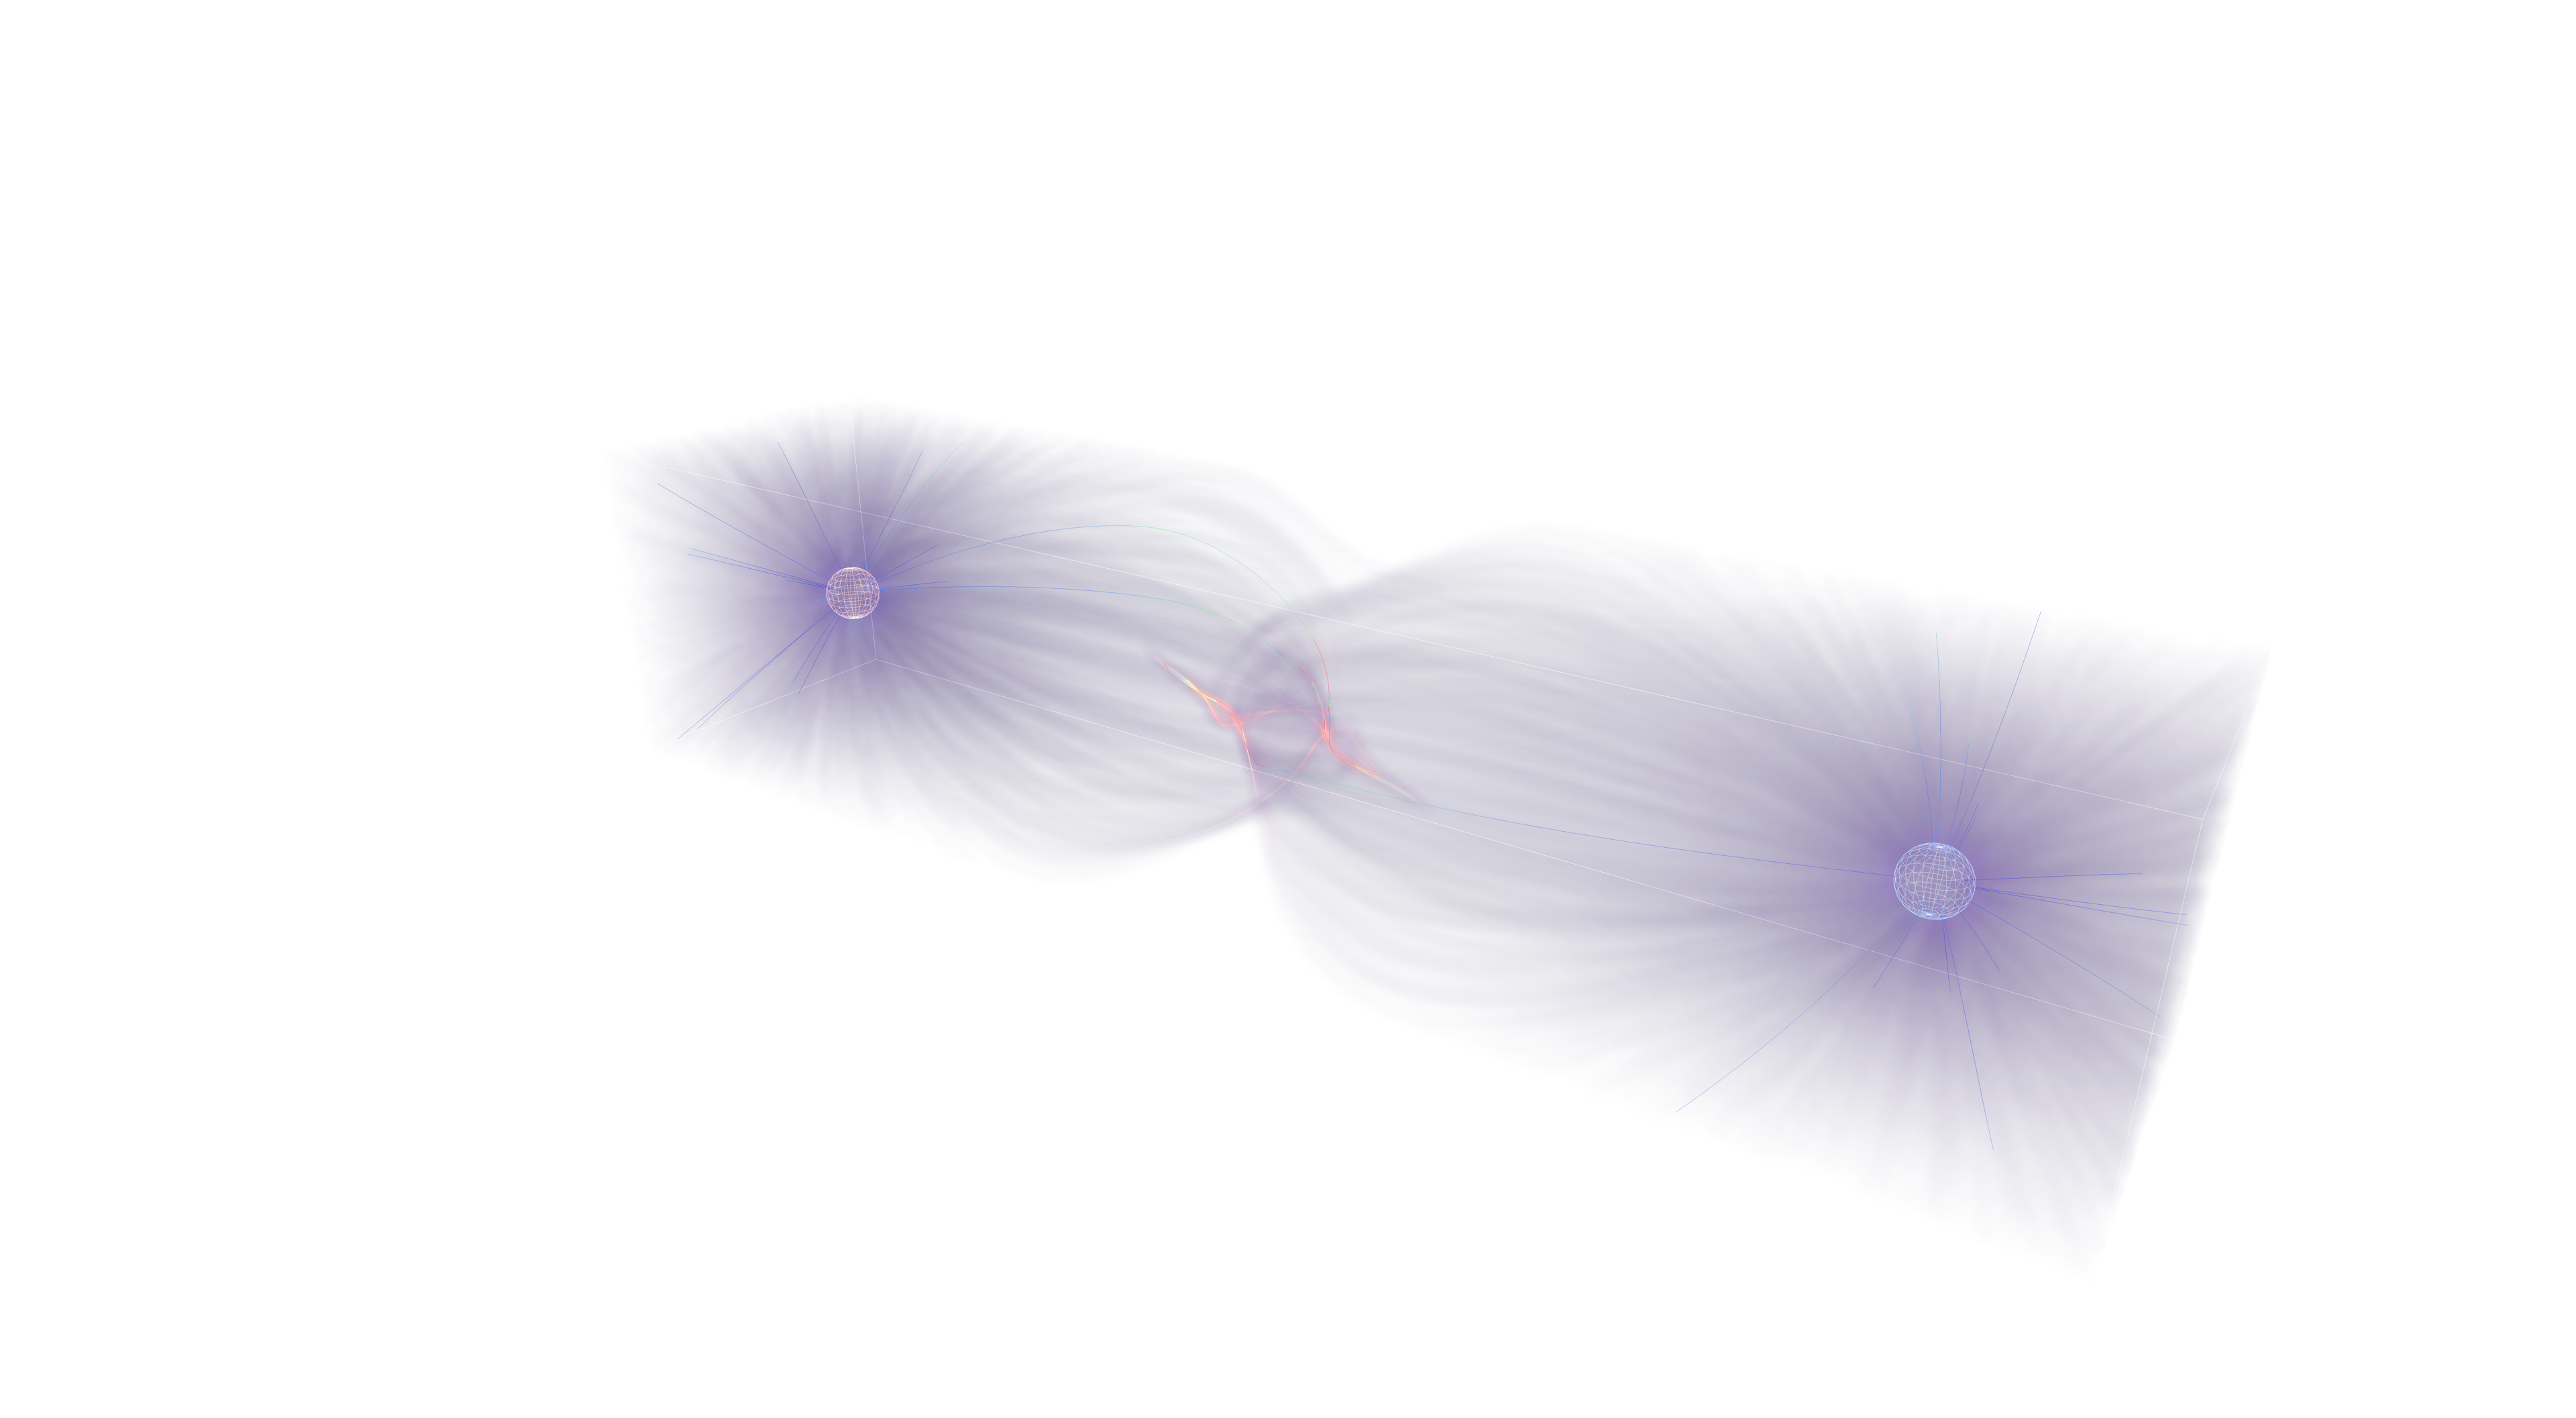
\includegraphics[width = 5 in]{2-emitter.png}
  \caption{
Two-emitter setup. 
}
\end{figure}

\begin{figure} 
\centering
  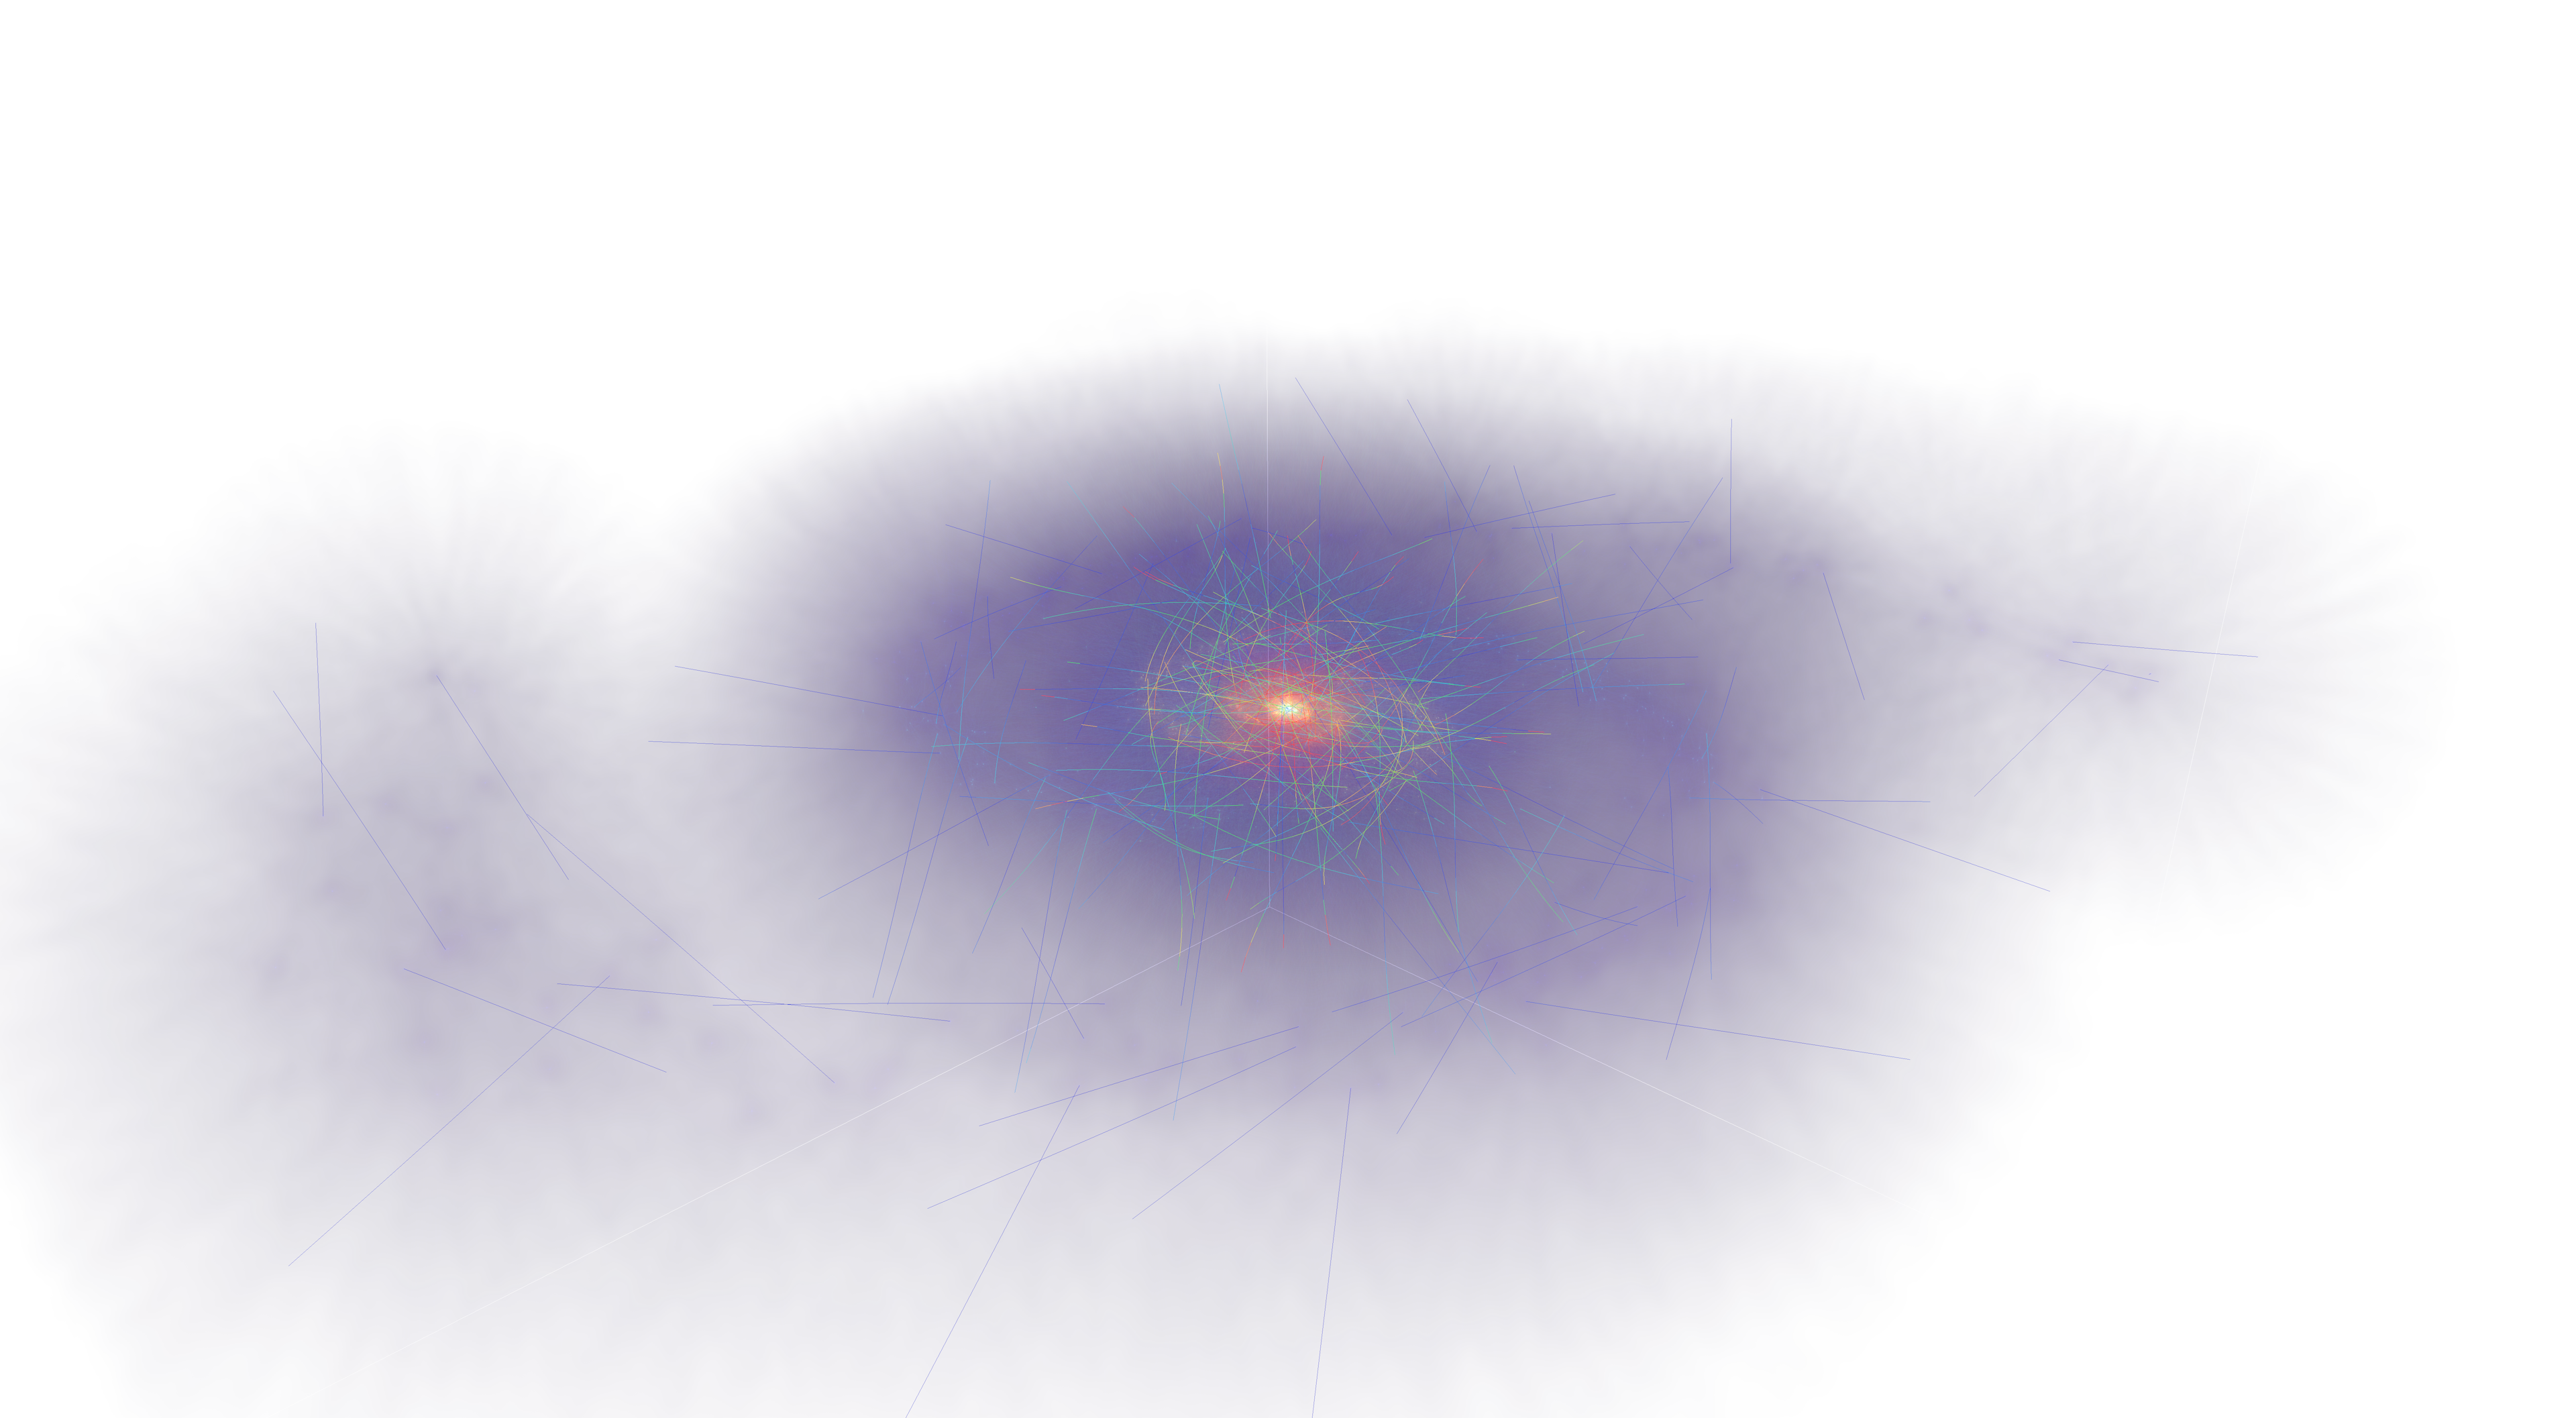
\includegraphics[width = 5 in]{galaxy.png}
  \caption{
Galaxy (many emitter) setup.
}
\end{figure}


\end{document}